	\begin{figure}[!h]
		\centering
 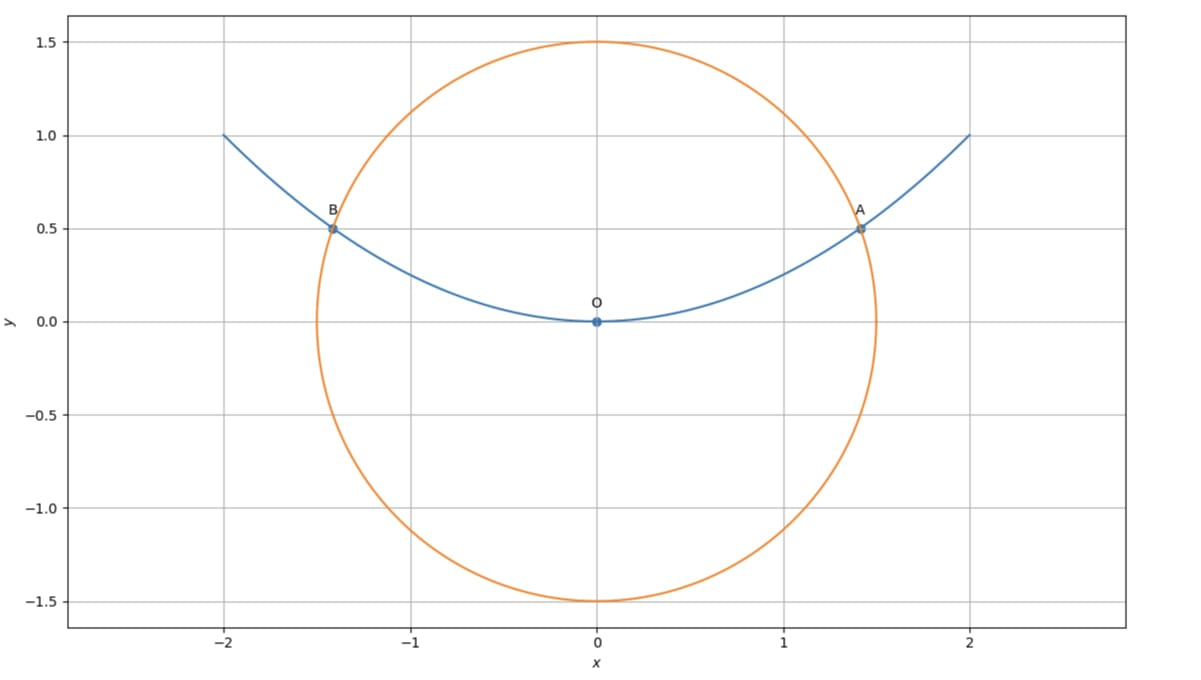
\includegraphics[width=\columnwidth]{chapters/12/8/2/1/figs/conic.jpg}
		\caption{}
		\label{fig:12/8/2/1}
  	\end{figure}
The given circle and parabola can be expressed as conics with parameters 
\begin{align}
	\vec{V}_1&=4\vec{I},
\vec{u_1}=\vec{0},
f_1=-9
\\
	\vec{V}_2&=\myvec{
1 & 0\\
0 & 0
},
\vec{u_2}= -\myvec{
0\\
2
},
f_2=0
\end{align} 
	  From \eqref{eq:pair-mat-sing-conic-det},
\begin{align}
\mydet{\mu+4 & 0 & 0\\ 
0 & 4 & -2\mu \\
0 & -2\mu & -9
} &= 0
\\
	\implies   \mu &= -4.
\end{align}
 Thus, the parameters for the pair of  straight lines can be expressed as 
 \begin{align}
	\vec{V} &= 
\vec{V}_1 + \mu\vec{V}_2
=\myvec{ 0 & 0 \\ 0 & 4},
\\
	\vec{u} &=
\vec{u}_1+\mu \vec{u}_2
	= \myvec{
0\\
8
    }
\\
	f&=-9,
	\\
	\implies \vec{D} &= \vec{V}, \vec{P} = \vec{I}
    \end{align}
On substituting
\begin{align}
\vec{q} &= \myvec{
0\\
0.5
} 
\end{align}
\begin{align}
\vec{m} = \myvec{2 \\ 0}
\end{align}
With the given Parabola,\\ 
\begin{align}
	\vec{V} &= \myvec{
1 & 0\\
0 & 0
    }
\end{align}
\begin{align}
	\vec{u} = -\myvec{2 \\0}
 \end{align}
 \begin{align}
  f = 0
 \end{align}
The value of $\kappa$ ,\\
\begin{align}
    \kappa = \sqrt{2},-\sqrt{2}
\end{align}
The points of intersection with Parabola along circle are \\
\begin{align}
    \vec{A}=\myvec{
\sqrt{2}\\
0.5
    }
\end{align}
\begin{align}
    \vec{B}=\myvec{
-\sqrt{2}\\
0.5
    }
\end{align}
 From the figure,
total area of portion is given by, 
\begin{align}
 A=  \int_{-\sqrt{2}}^{\sqrt{2}} g(x)-f(x) \,dx 
\end{align}
Where g(x) is area of circle and f(x) is the area of parabola around the points\\ 
\begin{align}
A= \int_{-\sqrt{2}}^{\sqrt{2}} \frac{\sqrt{9-4x^2}}{2}-\frac{x^2}{4} \,dx 
\end{align}
Area  
\begin{align}
    A= 3.0053609 \,m^2
\end{align}
